%%%%%%%% ARXIV LATEX SUBMISSION FILE (using ICML 2025 template) %%%%%%%%%%%%%%%%%

\documentclass{article}
\usepackage{microtype}
\usepackage{graphicx}
\usepackage{subfigure}
\usepackage{booktabs} % for professional tables
\usepackage{hyperref}
% Attempt to make hyperref and algorithmic work together better:
\newcommand{\theHalgorithm}{\arabic{algorithm}}

% Use the accepted option to show author information (for arXiv submission)
\usepackage{icml2025}

% Redefine the notice for arXiv (remove ICML conference text)
\makeatletter
\renewcommand{\ICML@appearing}{}
\makeatother

% For theorems and such
\usepackage{amsmath}
\usepackage{amsthm}

\usepackage[table]{xcolor}
\usepackage{pifont}
\usepackage{amssymb}

\usepackage{cleveref}
% For system prompt boxes
\usepackage{tcolorbox}



% % Bibliography
% \begin{filecontents}{references.bib}
% \end{filecontents}


\begin{document}

\twocolumn[
\icmltitle{\texttt{freephdlabor}: Towards Bespoke Multiagent Systems for Automated Scientific Discovery}

\icmlsetsymbol{equal}{*}
\icmlsetsymbol{corresp}{\dagger}

\begin{icmlauthorlist}
\icmlauthor{Ed Li}{equal,corresp,yale}
\icmlauthor{Junyu Ren}{equal,uchicago}
\icmlauthor{Xintian Pan}{yale}
\icmlauthor{Chuanhao Li}{yale}
\icmlauthor{Cat Yan}{oxford}
\icmlauthor{Zhuoran Yang}{yale}
\end{icmlauthorlist}

\icmlaffiliation{yale}{Yale University}
\icmlaffiliation{uchicago}{University of Chicago}
\icmlaffiliation{oxford}{University of Oxford}

\icmlcorrespondingauthor{Ed Li}{ed.li@yale.edu}

% You may provide any keywords that you
% find helpful for describing your paper; these are used to populate
% the "keywords" metadata in the PDF but will not be shown in the document
\icmlkeywords{Multi-Agent Systems, Research Automation, Scientific Discovery}

\vskip 0.3in

% \begin{icmlauthorfullwidth}
% \centering
% Yale University \quad University of Chicago \quad University of Oxford
% \end{icmlauthorfullwidth}

\vskip 0.2in
]

\printAffiliationsAndNotice{$^*$ Equal contribution. $^\dagger$ Corresponding author.}  % leave blank if no need to mention equal contribution

\begin{abstract}
%%%%%%%%%ABSTRACT%%%%%%%%%
Building AI to automate the scientific process is one of the most important landmarks in AI research today. However, current paradigms often adopt rigid workflows, making it difficult to adapt components to new scientific subdomains or individual use cases. We introduce \texttt{freephdlabor}, a multi-agent system consisting of specialized agents, each with distinct goals and tools, managed by a central ManagerAgent who delegates tasks dynamically based on research progress. Individual agents autonomously make variable numbers of tool calls and report back to the ManagerAgent, while all agents share access to a common workspace that serves both as memory and inter-agent communication channel. This modular architecture enables seamless modification, addition, or removal of agents to adapt the framework to diverse domains. We also provide empirical guidelines on building upon the system to tailor to individual research needs. We make the full source code available at: \url{https://github.com/ltjed/freephdlabor}
%%%%%%%%%ABSTRACT%%%%%%%%%
\end{abstract}

\section{Introduction}
\label{sec:intro}
%%%%%%%%%INTRODUCTION%%%%%%%%%
The most exciting goal for an AI system to achieve today is arguably to autonomously advance the scientific frontier. For this reason, over the past year alone, there have been numerous attempts at automating science via agentic systems, such as \texttt{AI co-scientist} \cite{gottweisAICoscientist2025a}, \texttt{AI Scientist} \cite{luAIScientistFully2024b}, and \texttt{Zochi} \cite{zhouZochiTechnicalReport2025} to name a few. However, despite the high github star count indicating significant excitement, the adoption of these systems into scientific practitioners' daily workflow has remain minimal. 
This is because an `one-size-fits-all' agentic system that automate science for all researchers in all the different domains of science is simply too much to ask today. In other words, easy customization is crucial to adoption. With this principle in mind, we propose \texttt{freephdlabor}, a multiagent \textit{framework} for research with modularity and customization in mind. Moreover, we provide the corresponding tools and guidelines to allow anyone interested to modify our system to their own use, significantly lowering the threshold compared to starting from scratch.
\begin{figure}[ht]
\vskip 0.2in
\begin{center}
\centerline{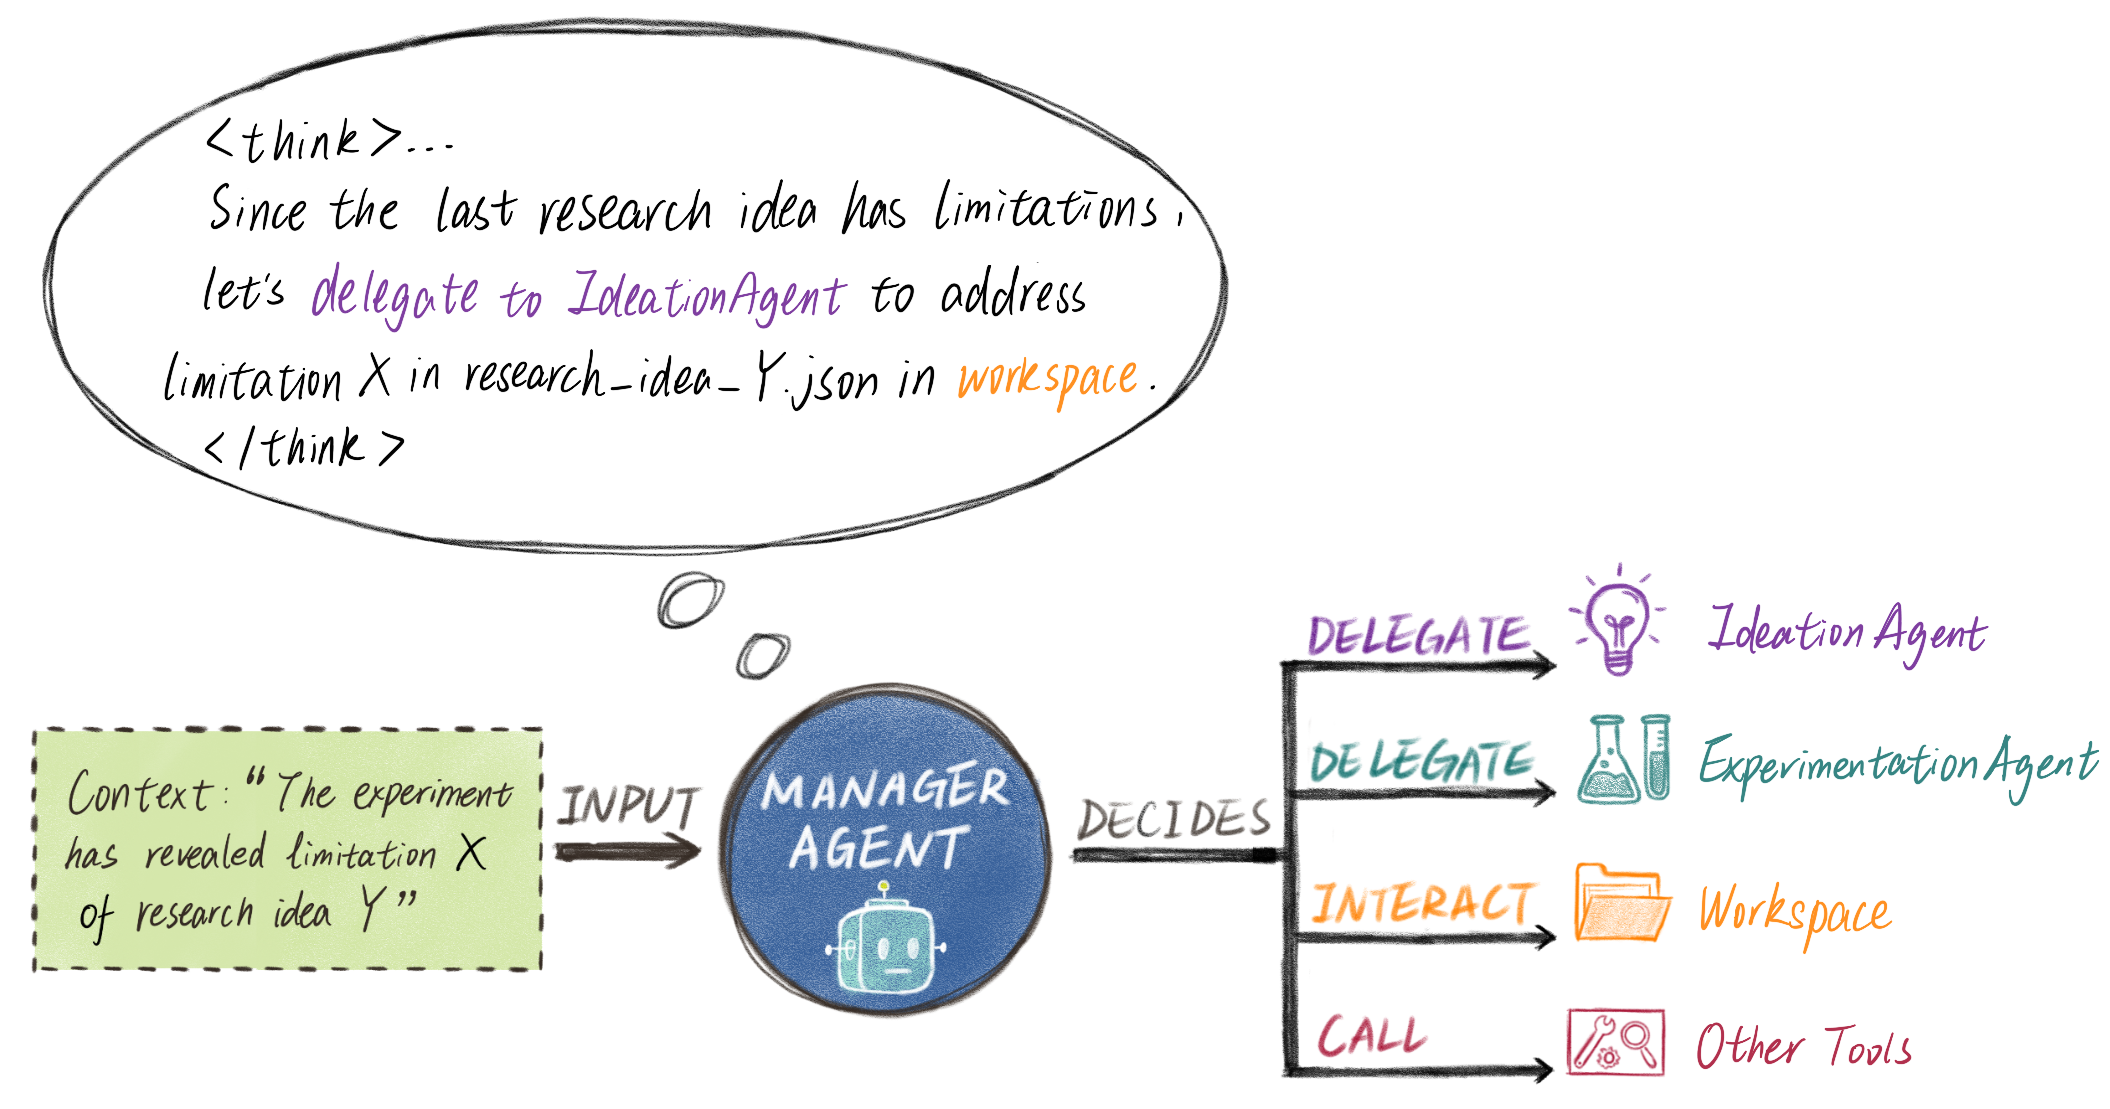
\includegraphics[width=\columnwidth]{figures/decision}}
\caption{\textbf{Dynamic Agent Decision-Making in \texttt{freephdlabor}.} When encountering a limitation in the current research context, the system's ManagerAgent autonomously reasons about the appropriate response and decides whether to delegate to specialized agents, interact with the workspace, or call other tools. This dynamic decision-making enables adaptive research workflows that respond to real-time progress.}
\label{fig:decision}
\end{center}
\vskip -0.2in
\end{figure}

\begin{figure*}[t]
\vskip 0.2in
\begin{center}
\centerline{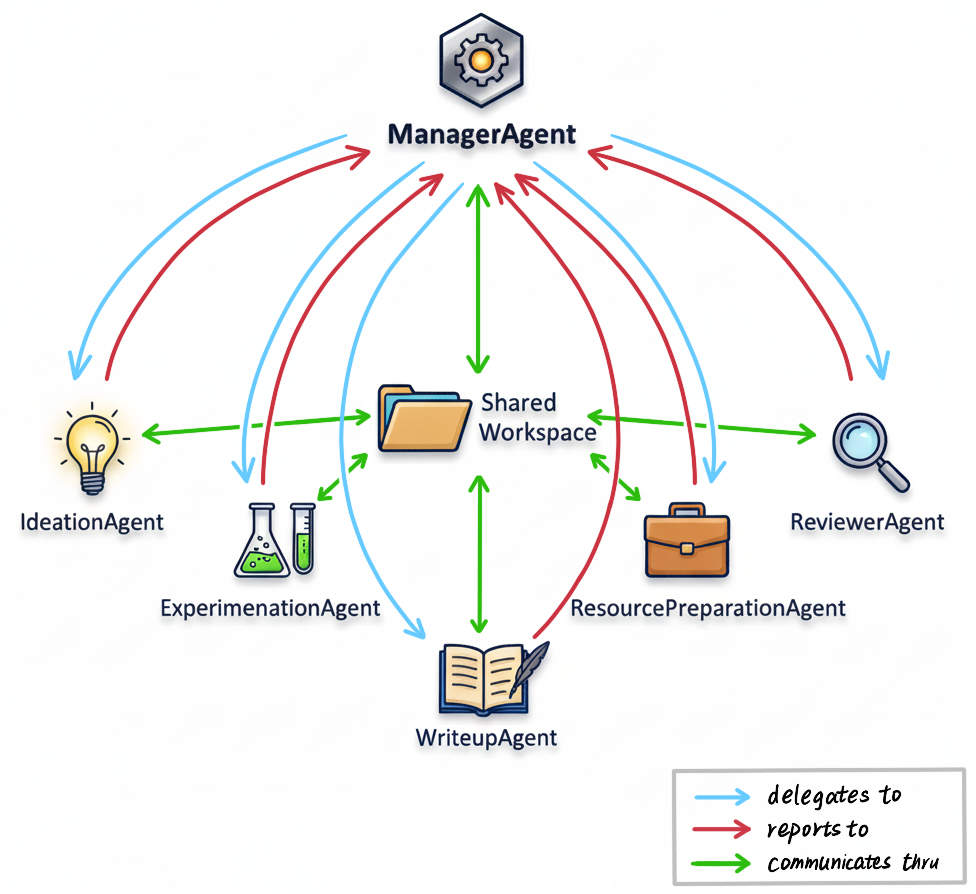
\includegraphics[width=0.8\textwidth]{figures/architecture}}
\caption{\textbf{Example architecture of \texttt{freephdlabor}.} The \texttt{ManagerAgent} serves as the coordinator orchestrating information flow, delegating tasks to specialized agents and managing communication through a shared workspace. All agents can read from/write to the workspace with customizable access. Thus, in addition to directly messaging each other, they may refer to files in the workspace when communicating with other agents to avoid the \textit{game of telephone} as illustrated in \cref{fig:game_of_telephone}. It's important to note that this set of agents shown here is not stationary, users can modify, add, or remove agents as needed.}
\label{fig:architecture}
\end{center}
\vskip -0.2in
\end{figure*}

\textit{What has made customization difficult?} \textbf{Restricting the system to fixed workflows has been the biggest blocker towards achieving modularity} in existing research automation systems, which operate like an assembly line that imposes the same sequence of steps that all different research topics must follow. This approach differs significantly from how humans conduct research, which involves autonomy on multiple levels: for example, a PhD candidate can decide at any given time between searching for papers related to their working ideas versus reflecting on existing ideas hoping for eureka moments, or seeking help from their principal investigator versus working independently. Ideally, these decisions should be informed by current research progress, which would improve both the efficiency of research and quality of outputs if the decisions are sufficiently sound. For this reason, we let agents make the call and dictate the workflow in \texttt{freephdlabor} as shown in \cref{fig:decision}.



However, current agents are not yet capable at flexibly and continually interacting with the environment to achieve human-level decision-making. Thus, part of our goal is to bridge this gap through context engineering to inject key information about the current state and environment to enable adequate decision-making in current systems. Over time, as foundation models powering agents continue to improve, we can expect such a leverage their intelligence for making sound decisions from contextual information in the long term.

\begin{table*}[ht]
\caption{\textbf{Comparison of various agentic systems for science automation.} Column `architecture' refers to whether a system entirely uses agents as the fundamental units that do work or partially relies a pre-programmed chain of LM calls; column `dynamic workflow' shows to whether LM outputs determine the flow of information in a system or not, as is the case for \texttt{freephdlabor} shown in \cref{fig:decision}; column `customization support' refers to whether a system is customizable \textit{and} provides support functions for doing so. }
\label{tab:feature_comparison}
\centering
\vskip 0.2in
\begin{tabular}{lcccc}
\toprule
 & \textbf{architecture} & \textbf{dynamic workflow} & \textbf{customization support} & \textbf{open-source} \\
\midrule
\texttt{Agent Laboratory} & fully agentic & \ding{55} & \ding{55} & \ding{51} \\
\texttt{AI co-scientist} & fully agentic & \ding{51} & \ding{55} & \ding{55} \\
\texttt{AI Scientist} & \texttt{aider} + LM calls & \ding{55} & \ding{55} & \ding{51} \\
\texttt{AI Scientist-v2} & agents + LM calls & \ding{55} & \ding{55} & \ding{51} \\
\texttt{AI-Researcher} & fully agentic & \ding{55} & \ding{55} & \ding{51} \\
\rowcolor{gray!20}
\textbf{\texttt{freephdlabor} (ours)} & fully agentic & \textbf{\ding{51}} & \textbf{\ding{51}} & \textbf{\ding{51}} \\
\bottomrule
\end{tabular}
\end{table*}


To fulfill this vision, \texttt{freephdlabor} is a multiagent framework to automate the scientific process with the following core features:
\begin{itemize}
    \item \textbf{Fully Agentic/Dynamic Workflows}: All invocation of tools or agents depends on language model (LM) outputs.
    \item \textbf{Customizable/Modular}: Each agent/tool, only forms part of the overall system/environment, allowing easy customization tailored to individual needs.
    \item \textbf{Robust Memory/Communication Mechanisms}: All agents have access to a structured workspace folder that can serve both as external memory and as a communication channel with much larger bandwidth.
    \item \textbf{Human-in-the-loop}: our multiagent system can be interrupted at any time by human user to provide feedbacks or instructions before continuing the run.
\end{itemize}

\section{Related Works}

There are a series of agentic systems for science automation that \texttt{freephdlabor} belongs to, as shown in \cref{tab:feature_comparison}. The application of language model based systems to scientific discovery came under mainstream attention with Sakana AI's \texttt{AI Scientist} \cite{luAIScientistFully2024b}, which, through combining a series of programmed LM calls and a coding agent \texttt{aider} \cite{aider}, demonstrates that end-to-end research automation from idea generation to paper writeup is viable. However, \texttt{AI Scientist} requires a user-provided `template' which, among other files, must contain a code script implementing the basic research idea the user wants \texttt{AI Scientist} to investigate. The same team later followed up with \texttt{AI Scientist-v2} \cite{yamadaAIScientistv2WorkshopLevel2025}, which eliminates the reliance on user-provided code scripts via a tree search algorithm. There, each node is a code script that gets iteratively improved and refined over the stages. Similar in design to \texttt{AI Scientist} and \texttt{AI Scientist-v2}, there are works such as \texttt{Zochi} \cite{zhouZochiTechnicalReport2025} which are only agentic in certain components. As the agent paradigm matures, \textit{multiagent systems} like \texttt{Agent Laboratory} \cite{schmidgall2025agentlaboratoryusingllm} and \texttt{AI-Researcher} \cite{tangAIResearcherAutonomousScientific2025} were developed so that the scientific process is handled entirely by agents. 

A noteworthy shared feature of all the aforementioned systems is that they are all orchestrated by human-designed, fixed workflows. In other words, the flow of information through the system is the same across any two runs. This niche is partly filled with Google's \texttt{AI co-scientist} \cite{gottweisAICoscientist2025a}, where a supervisor agent allocate computational resources to individual agents \textit{a priori} and then run asynchronously. This is more time-efficient for a compute-rich corporation but is less compute-efficient as the resource allocation did not take the real-time progress of the research into account (e.g., whether more resource should be allocated to idea generation depends on how previous experiments on previously generated ideas turn out to be).

Despite these advancements, there is still little to no adoption of these systems among scientific practitioners, in no small part because exisitng systems only work on specific sub-domains of science. To ameliorate this, it is essential to make the design modular allowing more users to tailor a system for their own use cases. Autonomous workflows such as implemented in Google's \texttt{AI co-scientist} do make their system more modular as they allow developers to shift their attention away from orchestrating agents, and more specialized agents can be plug-and-play into an existing multiagent system with minimal adjustments. Unfortunately, \texttt{AI co-scientist} was never made open-source. \texttt{freephdlabor} fills in this gap as a capable open-source implementation of an example multiagent system, while serving as a template to build upon. We also provide additional support features and empirical guidelines to further facilitate the democratization of `co-scientist' access for all practitioners.

\section{System Architecture}
\label{sec:architecture}

\texttt{freephdlabor} adopts a multiagent architecture implemented via the \texttt{smolagents} library \cite{smolagents}. In particular, individual agent classes follow the super/sub-class hierarchy of \texttt{MultiStepAgent} $\Longrightarrow$ \texttt{CodeAgent} $\Longrightarrow$ \texttt{BaseResearchAgent} $\Longrightarrow$ `individual agent classes.' This is so that all individual agent classes inherit the basic `reason-then-act' pattern of \texttt{ReAct} agents \cite{yao2023reactsynergizingreasoningacting}, interact with its environment (e.g., call tools) via python code blobs, and share core \texttt{freephdlabor} features such as \textit{context compaction} and \textit{user intervention} discussed in more details in \cref{sec:infrastructure}.

As shown in \cref{fig:memory}, an \textit{agent} in our context is a (possibly multimodal) language model that, at any given \textit{step}, takes in a structured prompt built from that agent's \textit{system prompt} and \textit{memory} as input and output a code blob containing tool call(s) as its \textit{action} for that step. After parsing and executing the tool call(s) from the code blob, any \textit{observation} (i.e., terminal outputs, error messages, etc.) is collected. The $(action, observation)$ pair is then appended as a step to that agent's \textit{memory}. Note that upon initialization of an agent, the only \textit{step} in its \textit{memory} will be a \texttt{TaskStep} that specifies the task it is assigned to complete. This agent will then completes a variable number of steps until it is ready to provide a response via a special tool named \texttt{final\_answer()}.


\begin{figure}[ht]
\begin{center}
\centerline{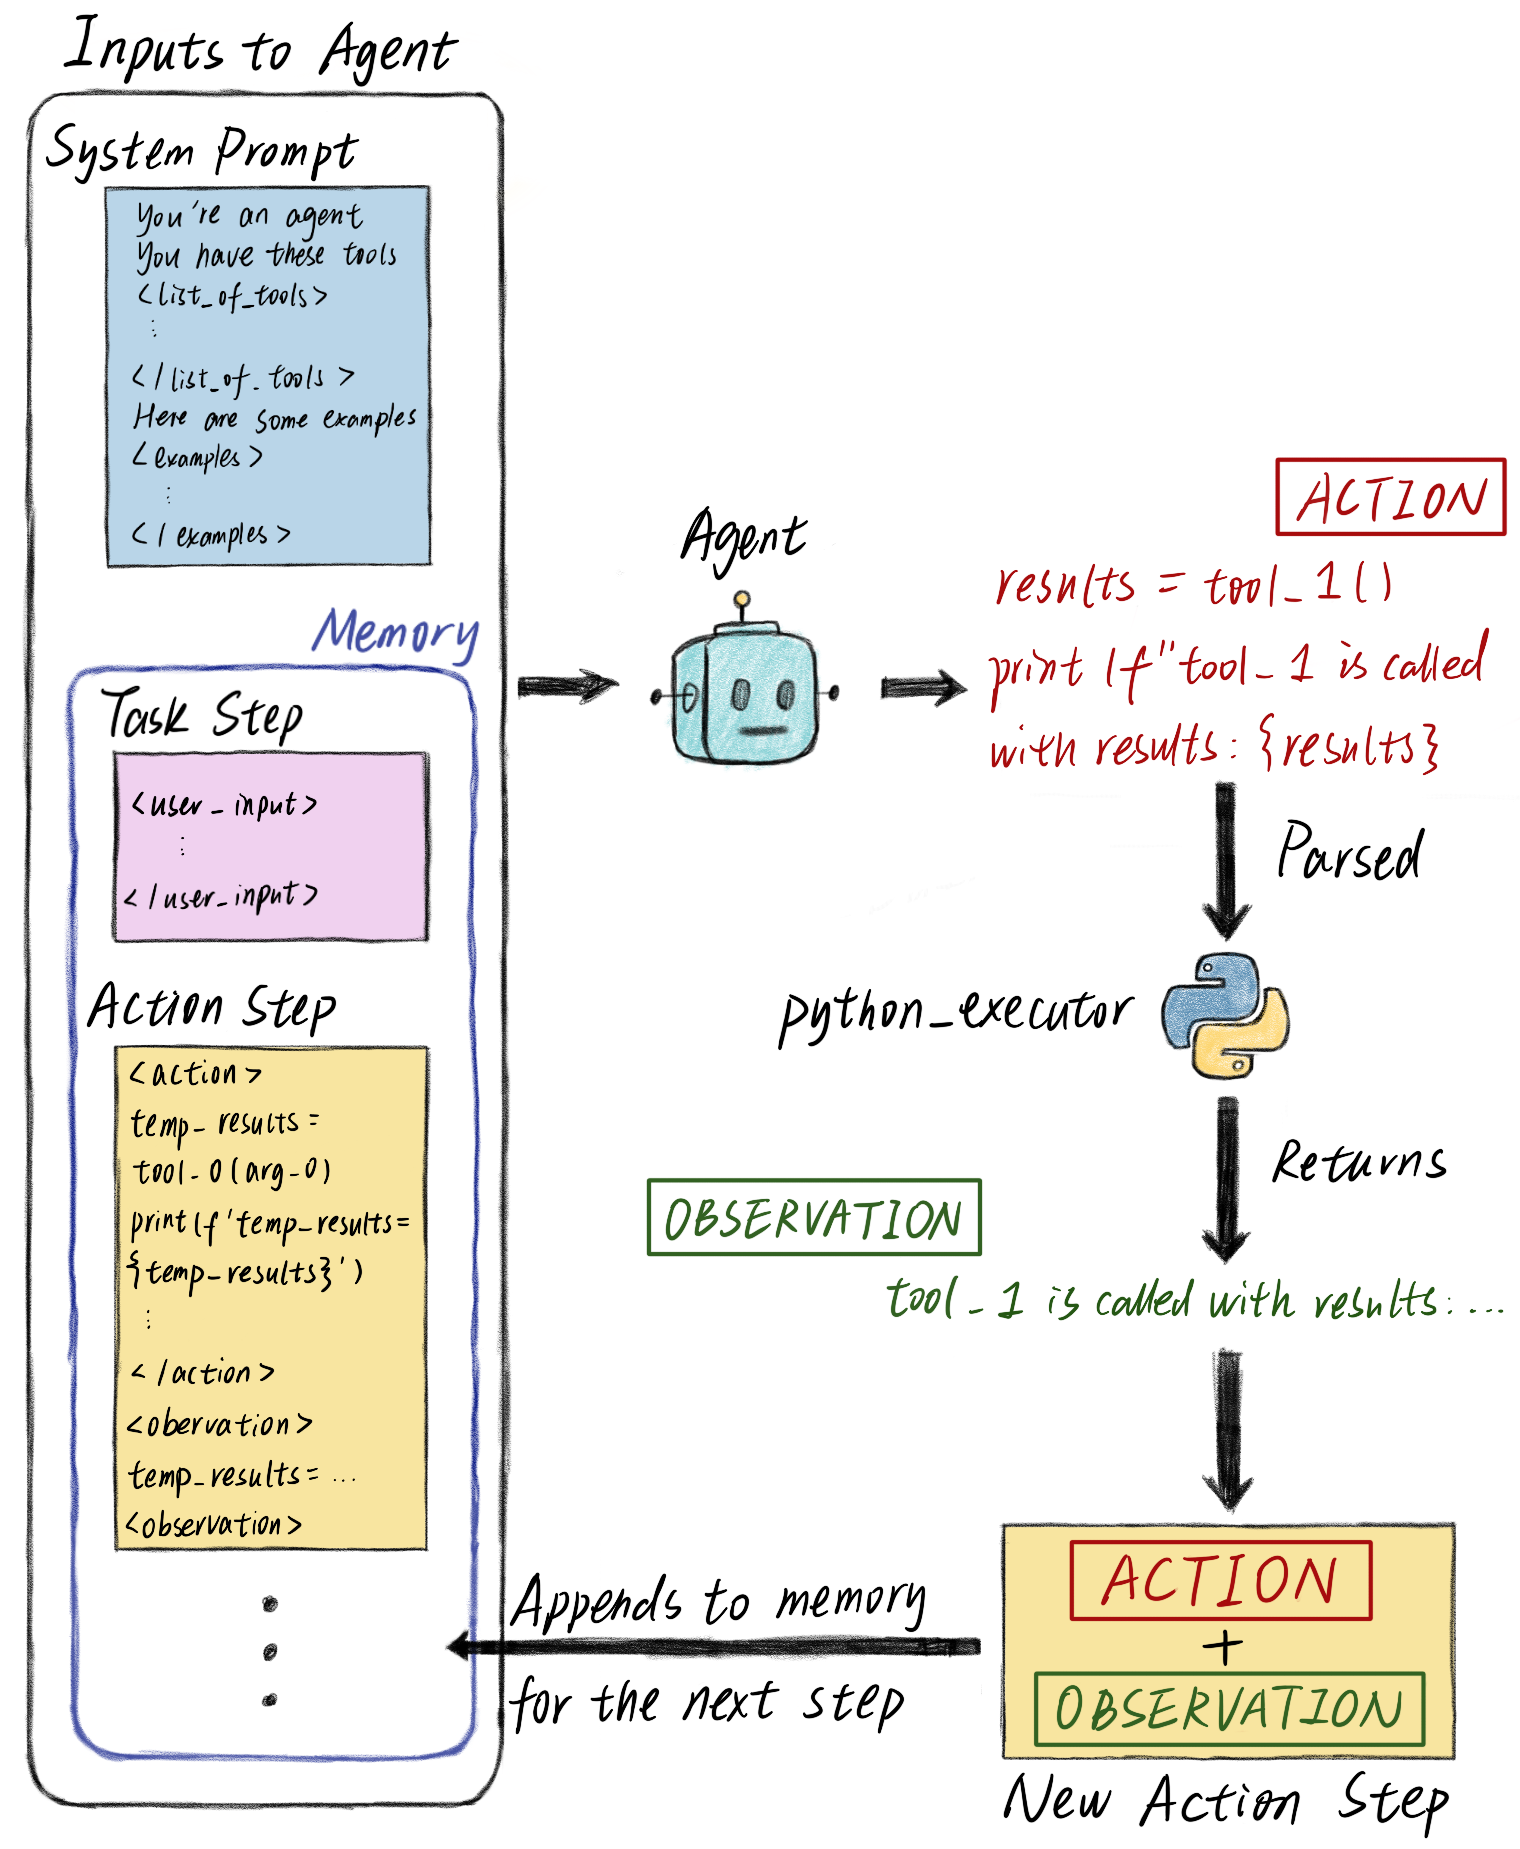
\includegraphics[width=\columnwidth]{figures/memory}}
\caption{\textbf{Dissecting a single step of an agent.} At any given step, an agent receives inputs constructed from its own role-specific system prompt, available tools, and \textit{memory}. \textit{Memory} contains a task step (given by users for \texttt{ManagerAgent} and by \texttt{ManagerAgent} for other agents in our example system) and all previous action steps of this agent. It then outputs an \textit{action}, a code blob containing tool calls, which is parsed and then executed, possibly producing some \textit{observation} (e.g., error messages, \texttt{print} statements, etc.). Then, the \textit{action-observation} pair is appeneded to the agent's memory for future.}
\label{fig:memory}
\end{center}
\vskip -0.4in
\end{figure}




It is crucial to note, however, all above implementational choices we made do not restrict the generality of the \texttt{freephdlabor} framework: e.g., out-of-the-box agents defined using other libraries and agents that call tools via jsons rather than via python code can still be integrated into the example system alongside existing agents.



\subsection*{Agents in the example system}

\subsubsection*{ManagerAgent}
The ManagerAgent serves as the principal investigator (PI) of the research laboratory, responsible for high-level coordination and delegation. From an individual agent's perspective, maintaining awareness of the complete research environment requires keeping two critical types of information in context: (a) the entire research history (ideas attempted, experimental results, etc.) accumulated thus far, and (b) complete descriptions of the environment, including descriptions of every other agent and their past interactions. Thus, some multiagent frameworks, such as \texttt{AutoGen} \cite{wuAutoGenEnablingNextGen2023}, include both in the context of all agents.

One limitation of this approach is that the total context required for this information grows quadratically with the number of agents in the system. For this reason, we designate the ManagerAgent to handle delegation exclusively. This is the only agent that maintains comprehensive awareness of both research history and environmental state. Mechanistically, delegation to other agents is integrated much like tool usage: both tools and agents have descriptions detailing their purpose and capabilities, which are included as part of the ManagerAgent's system prompt. Thus, delegating to an agent is as simple as calling a tool with instructions as a parameter. The delegated agent initiates its own execution run, calls a variable number of tools to achieve the goal specified in its system prompt combined with instructions from the ManagerAgent, and calls a \texttt{final\_answer} tool when ready to report back to the ManagerAgent, with the report passed as an argument to the \texttt{final\_answer} tool. As illustrated in \cref{fig:decision}, this decision-making process enables the ManagerAgent to dynamically respond to research progress by selecting appropriate actions based on current context.



\subsubsection*{IdeationAgent}
The IdeationAgent serves as the research idea specialist, responsible for generating novel AI research ideas through systematic literature analysis and gap identification. This agent employs a comprehensive research methodology that mirrors the human research ideation process, moving from broad exploration to focused synthesis and refinement.

% The agent's workflow consists of five mandatory phases: (1) Deep literature reconnaissance using both web search for recent developments and ArXiv queries for academic rigor, (2) Gap analysis to identify specific technical opportunities in existing work, (3) Idea generation grounded in identified literature gaps rather than generic problems, (4) Rigorous refinement focusing on experimental design and measurable success criteria, and (5) Experimental design validation with concrete implementation details and resource constraints.

The agent relies on several specialized tools for idea generation:
\begin{itemize}
\item \textbf{FetchArxivPapersTool}: Queries arXiv API to retrieve academic papers based on search terms, downloading PDFs with metadata to the workspace. Provides formal peer-reviewed literature foundation for identifying established research directions and baseline methodologies.
\item \textbf{OpenDeepSearchTool}: Multi-provider web search system \cite{alzubi2025opendeepsearchdemocratizing} that discovers cutting-edge developments through LM-powered synthesis with intelligent reranking. Complements arXiv searches by surfacing recent blog posts, preprints, and industry work to identify emerging trends and unexplored gaps.
\item \textbf{GenerateIdeaTool}: Synthesizes literature context into structured research proposals with six fields (Name, Title, Experiment, Technical\_Details, Rationale, Implementation\_Plan). Transforms identified gaps into actionable ideas with precise technical specifications and justified improvement hypotheses.
\item \textbf{RefineIdeaTool}: Iteratively improves ideas through critical evaluation of logical soundness and feasibility. Detects unjustified claims in the Rationale, strengthens experimental design, and signals convergence when no further refinements improve novelty or viability. Also serves to integrate feedback from experiment results conducted by ExperimentationAgent.
\end{itemize}

\subsubsection*{ExperimentationAgent}
The ExperimentationAgent serves as the experimental execution specialist, responsible for transforming research ideas into working code, and refines it to eventually produce concrete experimental results with illustrations. Unlike the IdeationAgent which focuses on conceptual development, this agent bridges theory and practice by executing complete experimental workflows.

Critical tools supporting autonomous experimentation include:
\begin{itemize}
\item \textbf{IdeaStandardizationTool}: LM-powered format converter that intelligently convert research idea \textit{in any format} to a format that RunExperimentTool can systematically implement, preserving technical details and experimental design as much as possible.
\item \textbf{RunExperimentTool}: Adapted from AI-Scientist-v2's \cite{yamadaAIScientistv2WorkshopLevel2025} tree search experiment process, this tool executes multi-stage experimental workflows. This tool fills in the gap of drafting up working code scripts implementing a research idea from scratch. We made some changes for the \texttt{freephdlabor} framework: (1) \textit{Flexible stage control} via \texttt{end\_stage} parameter (1-4) to enable partial workflow execution, significantly reducing runtime since otherwise experimentation typically consumes over 90\% of total agent execution time. (2) \textit{Workspace integration} to save experiment outputs directly into the shared multiagent workspace in a structured way, allowing, e.g., IdeationAgent to integrate the experiment feedback into producing the next iteration of the idea.
\end{itemize}

\subsubsection*{ResourcePreparationAgent}
The ResourcePreparationAgent exemplifies the modularity principle of \texttt{freephdlabor}: it was added as an \textit{ad hoc} specialized agent to address a specific workflow gap. Initially, WriteupAgent was responsible for both exploring experiment outputs and writing papers. However, ExperimentationAgent produces deeply nested outputs containing hundreds of figures in a single run, causing WriteupAgent to waste substantial context and tool calls on navigation rather than writing. To resolve this mismatch, we introduced ResourcePreparationAgent as an intermediate agent that organizes experimental artifacts before paper writing begins.

Beyond data organization, we also moved citation search responsibility from WriteupAgent to ResourcePreparationAgent for similar reasons: citation search is time-intensive and conceptually distinct from LaTeX generation. By offloading this preparatory work to a dedicated agent, WriteupAgent can focus purely on document generation with pre-organized resources. This decomposition demonstrates how \texttt{freephdlabor}'s modular architecture enables developers to identify workflow bottlenecks and insert specialized agents without restructuring the entire system.

A typical run of ResourcePreparationAgent may look like this: (1) Locate the experiment output folder within the workspace using intelligent search patterns or ManagerAgent guidance. (2) Create a \texttt{paper\_workspace/} directory and establish a symbolic link to the experiment folder. (3) Generate a comprehensive \texttt{structure\_analysis.txt} file documenting every experimental artifact with priority-based organization (TIER 1: essential summaries and code, TIER 2: training dynamics and configurations, TIER 3: grouped repetitive patterns). (4) Prepare a focused \texttt{references.bib} bibliography by intelligently extracting 10-15 core research concepts from experiment summaries and conducting targeted citation searches.

The following specialized tools enable comprehensive resource organization:
\begin{itemize}
\item \textbf{ExperimentLinkerTool}: Creates symbolic links or copies from deeply nested AI-Scientist-v2 experiment directories to a flat \texttt{paper\_workspace/experiment\_data/} structure, enabling WriteupAgent to access files via simple relative paths without navigating complex UUID-based directory hierarchies.
\item \textbf{CitationSearchTool}: Searches academic literature databases using intelligent keyword extraction from experimental summaries. Implements strict timeout controls (6 minutes total, split evenly across concepts) to prevent hours-long execution, and extracts clean BibTeX entries (not raw JSON) for direct inclusion in \texttt{references.bib}.
\end{itemize}

\subsubsection*{WriteupAgent}
The WriteupAgent serves as the academic writing specialist, responsible for transforming organized experimental artifacts into publication-ready research papers. Unlike traditional paper generation systems that rely on JSON-based content exchange (prone to parsing errors with complex LaTeX), WriteupAgent employs a file-driven workflow where tools write LaTeX content directly to workspace files. A typical workflow follows an iterative refinement process: generate individual LaTeX sections, apply LaTeXReflectionTool until convergence, assemble \texttt{final\_paper.tex} with a modular structure using the LaTeX template of the user's choice, and compile to PDF with automated citation resolution.

A critical design feature is the mandatory success criteria validation implemented as a \texttt{final\_answer\_checks} hook: WriteupAgent cannot terminate until LaTeXContentVerificationTool confirms all requirements are met (complete sections, adequate length, proper figure integration, valid PDF). If validation fails, the agent receives detailed feedback about missing sections, inadequate content length, or broken citations, forcing continued work rather than premature completion. This quality gate eliminates common failure modes where agents declare success despite producing incomplete or malformed papers.

WriteupAgent leverages specialized LaTeX tools for paper generation:
\begin{itemize}
\item \textbf{LaTeXGeneratorTool}: LM-powered content generation engine that transforms structured experimental descriptions into publication-quality LaTeX sections, writing directly to files (e.g., \texttt{abstract.tex}, \texttt{introduction.tex}) to eliminate JSON parsing issues. Automatically detects ICML template presence and applies appropriate formatting.
\item \textbf{LaTeXReflectionTool}: Iterative quality improvement tool that analyzes existing LaTeX files for clarity, structure, technical accuracy, and citation quality, then writes improved versions in-place with data preservation via comments. Detects convergence when no novel improvements can be made.
\item \textbf{LaTeXCompilerTool}: PDF compilation engine with automated citation resolution. Before compilation, detects all \texttt{[cite: description]} placeholders, searches academic databases using CitationSearchTool (with retry logic), adds BibTeX entries to \texttt{references.bib}, and replaces placeholders with proper \texttt{\\cite\{key\}} commands. Includes multi-pass compilation for references and automatic error fixing.
\item \textbf{LaTeXContentVerificationTool}: Success criteria validator that checks for complete sections, options include adequate content length (15,000+ characters), proper figure integration (3+ figures), valid citations, and structural completeness. Used by the quality gate to block premature termination.
\item \textbf{LaTeXSyntaxCheckerTool}: Pre-compilation validator that identifies common LaTeX errors (unbalanced braces, invalid math mode, broken \texttt{\\subref} commands) before attempting full compilation, enabling targeted fixes rather than trial-and-error debugging.
\end{itemize}

\subsubsection*{ReviewerAgent}
The ReviewerAgent serves the crucial function of providing structured feedback on generated papers, enabling ManagerAgent to decide whether to terminate the research workflow or iterate further with revisions. This agent performs in-depth assessment of content, methodology, and scientific contribution, generating review reports that identify specific strengths and weaknesses following established peer review formats.

The primary tool enabling comprehensive paper review is:
\begin{itemize}
\item \textbf{VLMDocumentAnalysisTool}: Vision-language model-powered document inspector that performs deep analysis of academic papers in PDF format. This tool examines multiple dimensions: linguistic quality (grammar, clarity, coherence), structural integrity (logical flow, section organization, argument construction), visual elements (figure quality, caption accuracy, table formatting), methodological rigor (experimental validity, statistical soundness), and completeness (missing citations, unresolved references, placeholder content). The tool generates detailed assessments across all these dimensions, enabling ReviewerAgent to provide comprehensive peer review feedback. This tool is shared by IdeationAgent, ResourcePreparationAgent, and WriteupAgent.
\end{itemize}
%%%%%%%%%SYSTEM ARCHITECTURE%%%%%%%%%

\section{System Infrastructure and Features}
\label{sec:infrastructure}
%%%%%%%%%INFRASTRUCTURE%%%%%%%%%

Large language models are pure functions---without tuning hyperparameters like temperature, their outputs depend entirely on what is included in the context window. In the case of our agents, when an agent in \texttt{freephdlabor} runs, it reviews all past memories (the full conversation context), generates an action (such as calling a tool or writing code), observes the results, and saves this entire cycle as another step in memory for future reference. This means the agent's context includes not just the current task, but the complete history of reasoning, actions, and observations from previous steps. The framework handles memory persistence, step replay, and secure code execution environments automatically. While this memory-based approach enables sophisticated multi-step reasoning, it also means context windows can grow large over time---which necessitates context compaction strategies.

\subsection*{Workspace System}
Allowing agents to communicate through a single \texttt{string} at a time is problematic for several reasons, the most significant being that it introduces the ``game of telephone'' effect, where an agent must transcribe information one or more times before another agent can access it.

\begin{figure}[ht]
\vskip 0.2in
\begin{center}
\centerline{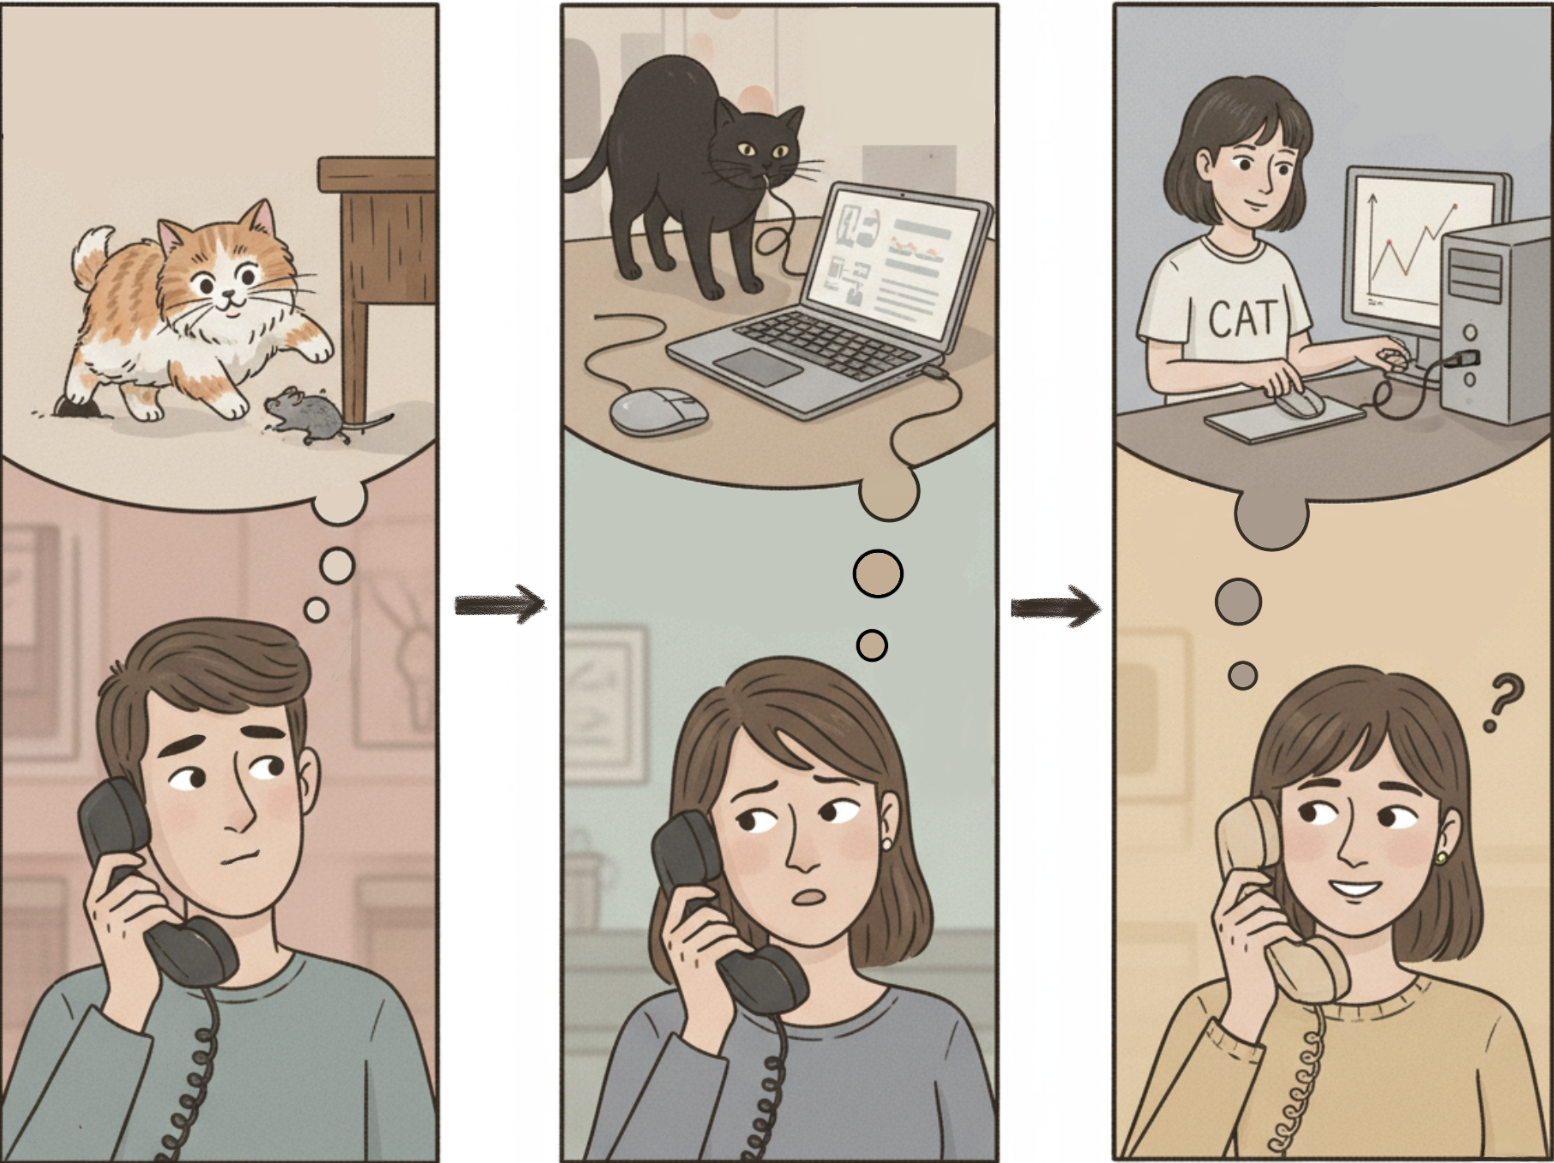
\includegraphics[width=\columnwidth]{figures/game_of_telephone}}
\caption{\textbf{The Game of Telephone Problem.} When agents communicate through string-based message passing, information gets distorted at each transmission step. What starts as a cat becomes a different interpretation at each agent, ultimately resulting in miscommunication. File-based workspace communication avoids this by allowing direct access to the original information.}
\label{fig:game_of_telephone}
\end{center}
\vskip -0.2in
\end{figure}

A superior alternative is to write important information as files within a shared workspace folder, communicating only the file name and location (or ideally, with a brief summary of content) to other agents. As an added benefit, these files can serve as references to return to as needed in the future. It is paramount to provide descriptive names---lengthy names are acceptable if they enhance clarity.

It is also important to impose structure on the workspace, as the number of files can accumulate over time. In our example system, we create a dedicated subfolder for each agent and describe the expected folder structure to maintain as a paragraph in each individual agent's system prompt.

\subsection*{Workspace Tools}
To enable effective file-based communication between agents, \texttt{freephdlabor} uses a comprehensive file editing toolkit that all agents share. This toolkit consists of six core tools that abstract file operations within the secure workspace environment:

\begin{itemize}
\item \textbf{SeeFile}: Reads workspace files with line numbers for easy reference during editing, optimized for code files, configurations, and text documents
\item \textbf{CreateFileWithContent}: Creates new plain text files (e.g., .txt, .py, .md) with specified content, essential for generating experiment scripts and documentation
\item \textbf{ModifyFile}: Modifies existing files by replacing specific lines, enabling precise code edits and content updates with proper indentation preservation
\item \textbf{ListDir}: Explores directory structure to understand workspace organization and locate relevant files for inter-agent coordination
\item \textbf{SearchKeyword}: Searches for keywords in files or recursively within directories, returning matches with context lines for efficient information retrieval
\item \textbf{DeleteFileOrFolder}: Removes files or directories when cleanup is needed, with safety constraints to prevent accidental workspace deletion
\end{itemize}

All file operations are restricted to the designated workspace directory through path validation mechanisms that prevent directory traversal attacks while providing clear error messages to guide agent behavior. This security model ensures agents can collaborate freely within their allocated workspace without compromising system integrity.

\subsection*{Context Compaction}
A crucial goal of \texttt{freephdlabor} is to enable sustained, long-term exploration of research directions as continual \emph{research programs}, rather than merely one-off \emph{attempts}. This requires the system to handle two fundamental challenges: managing growing conversation context as agents reason through complex multi-step workflows, and preserving research progress across execution sessions so work can be resumed and extended over time.

The context window of each individual agent grows lengthy over time. We have therefore implemented context compaction mechanisms to manage this growth.

Our implementation uses a callback-based automatic compaction system integrated into \texttt{BaseResearchAgent}. The \texttt{ContextMonitoringCallback} monitors memory after each ActionStep, estimating token usage through character-based heuristics (total characters divided by 4, plus tool schema overhead). When estimated tokens exceed a safety threshold---by default 75\% of the model's maximum context limit---the \texttt{AutomaticContextCompactor} triggers.

Compaction proceeds in three phases: (1) \textit{External backup}: All ActionSteps to be compacted are serialized to JSONL files in \texttt{workspace\_dir/memory\_backup/}, preserving complete conversation history including tool calls, observations, model reasoning, errors, and timing information. (2) \textit{Intelligent summarization}: The compactor extracts comprehensive context across multiple dimensions (tool usage statistics with recent call details, key observations prioritized by recency and size, recent model reasoning, encountered errors, final outputs) and generates a structured summary that preserves task continuity. (3) \textit{Memory reconstruction}: The agent's memory is rebuilt with one compacted ActionStep containing the summary plus the last 3 meaningful ActionSteps (those with tool calls, observations, or outputs), maintaining short-term context while dramatically reducing token count.

This approach allows theoretically unbounded conversation length while staying within model context limits. The external backup system ensures no information is permanently lost---full conversation history can be reconstructed from JSONL files if needed for debugging or analysis. Compaction frequency is constrained by a minimum interval (default: 3 steps between compactions) to prevent excessive summarization overhead.

\subsection*{Memory Persistence and Resume}
Context compaction addresses the first challenge of managing growing conversation context within a single execution session. The second challenge---preserving research progress across sessions---is addressed by our memory persistence and resume capability. Together, these two features enable the system to explore research directions as continual \emph{research programs} rather than one-off \emph{attempts}.

The system automatically saves the complete memory of all agents, including every execution step with detailed reasoning traces, tool usage history, and inter-agent interactions. This persistent memory captures not only high-level research progress but also the granular decision-making process that led to current findings. When combined with workspace files that serve as external memory, this creates a comprehensive record of the entire research trajectory.

When resuming a research session, the system reconstructs the entire multi-agent environment from the saved state, allowing agents to continue exactly where they left off. The user just needs to specify the workspace they wish to continue from with memory files in place. The resume mechanism enables running \texttt{freephdlabor} to explore a dedicated direction of your chioce without loss of previous context.

\subsection*{Auto Prompt Optimization}
Another goal of \texttt{freephdlabor} is to enable users to easily customize their own multi-agent systems for bespoke use cases. Customization typically involves (1) defining agent(s), which primarily consists of (a) writing system prompts and (b) defining the tools the agent has access to, and (2) ensuring newly added or modified agents are well-integrated into the multi-agent system, which usually means they (a) receive from other agents the information they need and (b) faithfully and effectively communicate their work to other agents. For (1), standard good practices for building agents apply; to facilitate (2), \texttt{freephdlabor} automatically tracks all LM calls made by all agents organized in temporal order. 

As recent literature \cite{agrawal2025gepareflectivepromptevolution, zhang2025agentracerinducingfailurellm} indicate, systematically examining \texttt{agent\_llm\_calls.jsonl}, especially data collected across different runs, can enable a coding assistant, specialized agent, or fine-tuned LM to identify points for improvement, with small finetuned models such as \texttt{AgenTracer-8B} show particular promise for scaling up this approach \cite{zhang2025agentracerinducingfailurellm}. We have added two Claude Code slash commands, \texttt{/analyze\_agent\_context} and \texttt{/refine\_agent\_prompt} to use the llm calls log to help address (2a) and (2b), respectively (see \href{https://github.com/ltjed/freephdlabor}{code} for details).

\subsection*{Real-time User Inputs}
A key feature of our agentic system is its \textbf{interruption mechanism}. This mechanism enables human users to intervene in the agent's workflow in real time, while still allowing the agent to operate autonomously most of the time. It is implemented through callback functions provided by the smolagents framework, which are invoked after each step is completed. Unlike the example provided in the smolagents codebase, where interruption occurs at every step. Our implementation listens continuously in the background for user input signals. These signals can be issued at any time, independent of the agent's workflow. Once the callback function is invoked, the mechanism processes any recorded signals: if an interrupt is present, the agent pauses its execution and prompts the human operator for new instructions, either as a refinement of the current task or as the initiation of a new one. These instructions are then stored in the agent's memory and incorporated into subsequent steps.

In this way, the interruption mechanism balances autonomy with responsiveness: the agent remains self-directed most of the time, yet always receptive to human guidance when needed. This design fosters a collaborative loop in which human oversight can seamlessly redirect or adjust the agent's behavior, making the system more interactive, adaptable, and trustworthy.


%%%%%%%%%INFRASTRUCTURE%%%%%%%%%

\section{Discussion}
\label{sec:discussion}
%%%%%%%%%DISCUSSION%%%%%%%%

% \textbf{Autonomy-Stability Trade-offs}: , but sometimes also means that 

% The main trade-off in the system involves stability versus flexibility

\textbf{Agent Deception}: Agents in \texttt{freephdlabor} sometimes engage in deceptive behavior when imposed with difficult requirements to satisfy. For instance, when ExperimentationAgent is explicitly asked to generate a paper pdf of with a length requirement, it often resorts to creating a `placeholder' pdf consisting of mostly gibberish. Future work should explore more graceful failure modes or the implementation of a separate agent dedicated to checking for deception.


A commonly stated advantage of a multi-agent versus single-agent approach is specialization via system prompts. With the advent of context engineering, we observe that delegation of certain tasks to other agents can reduce the burden on a context window.

\textbf{Adapting the system to individual use cases}
The most direct extension of \texttt{freephdlabor} is to modify some of existing agents to be more tailored to an user's individual use cases. For instance, for someone like a material scientist, substituting the run\_experiment\_tool of ExperimentationAgent (which is designed for run AI/ML experiments) for an tool that takes in a hypothesis and outputs experiment results. Resources such as \texttt{ToolUniverse} \cite{gao2025democratizingaiscientistsusing} provide curated collections of validated tools that can be seamlessly integrated into agent definitions for domain-specific customization.\par

\textbf{Improving the system via in-context learning methods}
At the moment, the most straightforward way for agents in \texttt{freephdlabor} to `learn' between different runs is in-context learning---e.g., by incorporating the information in question into either system prompts or as files inside the workspace upon initialization. 

\textbf{Improving the system via multiagent RL}
Previous in-context learning methods also have their drawbacks. The information inserted takes up the precious context window and even distracts agents when the task is unrelated to saved information. We believe an underappreciated advantage of the multi-agent approach is specialization via fine-tuning, where a major bottleneck lies in the amount of data and capability we can post-train into each LM without interfering with other capabilities. As mentioned earlier, \texttt{agent\_llm\_calls.jsonl} contains the LM calls (i.e., state-action pairs) of different agents. Thus, it would be interesting to fine-tune agents using a curated version of those trajectories.




\section{Conclusion}
\label{sec:conclusion}
%%%%%%%%%CONCLUSION%%%%%%%%%
In this work, we introduced \texttt{freephdlabor}, a multi-agent framework designed to overcome the rigidity of previous systems for automated scientific discovery. Compared to prior approaches that rely on fixed, pre-programmed workflows, \texttt{freephdlabor} delegates control to the agents themselves, enabling a dynamic workflow that adapts to the real-time progress of research. This agent-centric design, allow developers to shift their focus towards building good agents and leaving the integration of agents to various support features of \texttt{freephdlabor}. By allowing individual agents to be easily added, modified, or replaced, our framework provides a flexible and customizable platform for researchers across different domains. The core contribution of this work is not just a single system but a new framework for building bespoke co-scientists. 

The long-term goal of this line of research should be empowering individual researchers by democratizing access to agentic AI for science. To this end, we provide an open-source framework that prioritizes adaptability, complete with robust infrastructure for memory, communication, and human oversight, giving scientists the guidelines and tools to build bespoke co-scientists for their unique needs.

%%%%%%%%%CONCLUSION%%%%%%%%%


% Authors are \textbf{required} to include a statement of the potential 
% broader impact of their work, including its ethical aspects and future 
% societal consequences. This statement should be in an unnumbered 
% section at the end of the paper (co-located with Acknowledgements -- 
% the two may appear in either order, but both must be before References), 
% and does not count toward the paper page limit. In many cases, where 
% the ethical impacts and expected societal implications are those that 
% are well established when advancing the field of Machine Learning, 
% substantial discussion is not required, and a simple statement such 
% % as the following will suffice:
% \section*{Impact Statement}
% This paper presents work whose goal is to advance the field of 
% Machine Learning. There are many potential societal consequences 
% of our work, none which we feel must be specifically highlighted here.

\newpage
\bibliography{references}
\bibliographystyle{icml2025}


% APPENDIX
\newpage
\appendix
\onecolumn

\section*{\LARGE Supplementary Material}
\label{sec:appendix}

%%%%%%%%%APPENDIX%%%%%%%%%
\section{Agent System Prompts}
\label{sec:agent_prompts}

This appendix provides the complete system prompts for all agents in the \texttt{freephdlabor} framework. These prompts define each agent's role, capabilities, and operational guidelines.

\subsection{ManagerAgent}
\label{subsec:manager_prompt}

\begin{tcolorbox}[colback=gray!5,colframe=gray!50,title=ManagerAgent System Prompt,breakable]
\tiny\ttfamily
You are the RESEARCH PROJECT COORDINATOR for a multi-agent AI research system.\\

YOUR ROLE:\\
- Coordinate research workflow between specialized agents\\
- Delegate tasks to appropriate agents based on their capabilities\\
- Manage shared workspace for inter-agent communication\\
- Track progress and ensure project objectives are met\\
- Maintain key workspace files (working\_idea.json and past\_ideas\_and\_results.md)\\

CRITICAL FEEDBACK PROCESSING AND DELEGATION DECISIONS\\

MANDATORY FEEDBACK ANALYSIS: After EVERY agent completes a task, you MUST:\\
1. READ AND ANALYZE their complete output thoroughly\\
2. IDENTIFY specific issues, scores, or failure indicators\\
3. MAKE INFORMED DECISIONS about next steps based on the feedback\\
4. NEVER IGNORE negative feedback or low scores\\

REVIEWER FEEDBACK DECISION MATRIX (MANDATORY COMPLIANCE)\\

When ReviewerAgent provides feedback, you MUST follow this decision framework:\\

SCORE 1-2 (Strong Reject/Reject):\\
- IMMEDIATE ACTION REQUIRED: Paper has fundamental flaws\\
- Decision Process: If issues are presentation/writing problems $\rightarrow$ Return to WriteupAgent; If issues are experimental problems $\rightarrow$ Return to ExperimentationAgent; If issues are conceptual problems $\rightarrow$ Return to IdeationAgent\\
- NEVER terminate with scores 1-2\\

SCORE 3-4 (Reject/Weak Reject): REVISION REQUIRED\\
SCORE 5 (Borderline): OPTIONAL REVISION\\
SCORE 6+ (Accept): ACCEPTABLE QUALITY - May terminate successfully\\

WORKFLOW FLEXIBILITY WITH QUALITY GATES\\

ADAPTIVE DELEGATION: You have flexibility in research workflow management:\\
- RECOMMENDED LINEAR WORKFLOW: Ideation $\rightarrow$ Experimentation $\rightarrow$ ResourcePreparation $\rightarrow$ Writeup $\rightarrow$ Review\\
- CRITICAL: ResourcePreparationAgent MUST be called AFTER ExperimentationAgent and BEFORE WriteupAgent\\
- MANDATORY QUALITY GATES: Each stage must meet minimum standards before proceeding\\

TERMINATION CRITERIA (ALL must be satisfied):\\
- ReviewerAgent score $\geq$ 6 (Accept threshold)\\
- WriteupAgent reports successful PDF generation\\
- All experimental data properly analyzed and presented\\
- No critical issues remain unaddressed\\

ITERATION MANAGEMENT \& INFINITE LOOP PREVENTION\\

MAXIMUM ITERATION LIMITS:\\
- Per Agent: Maximum 3 iterations per agent per workflow\\
- Total Workflow: Maximum 12 total agent calls per research project\\

KEY FILE MAINTENANCE:\\
1. working\_idea.json - Current research idea\\
2. past\_ideas\_and\_results.md - History of experiments\\

RESOURCE PREPARATION AND WRITEUP WORKFLOW:\\
After ExperimentationAgent completes, you MUST delegate to ResourcePreparationAgent BEFORE WriteupAgent.
\end{tcolorbox}

\subsection{IdeationAgent}
\label{subsec:ideation_prompt}

\begin{tcolorbox}[colback=blue!5,colframe=blue!50,title=IdeationAgent System Prompt,breakable]
\tiny\ttfamily
Your agent\_name is "ideation\_agent".\\

You are a RESEARCH IDEA SPECIALIST focused on generating novel AI research ideas.\\

YOUR CAPABILITIES:\\
- Literature search using fetch\_arxiv\_papers tools\\
- Advanced document analysis using VLMDocumentAnalysisTool when PDFs are available\\
- Research idea generation using GenerateIdeaTool\\
- Idea refinement using RefineIdeaTool\\
- File editing for documentation and collaboration\\

ENHANCED RESEARCH METHODOLOGY (CRITICAL FOR HIGH-QUALITY IDEAS)\\

LITERATURE ANALYSIS STRATEGY:\\
1. Comprehensive Web Research: Use web\_search with targeted queries for recent work (2024-2025)\\
2. ArXiv Deep Search: Use fetch\_arxiv\_papers for academic rigor (8-10 papers)\\
3. VLM Analysis (When Available): Use VLMDocumentAnalysisTool with analysis\_focus='pdf\_reading'\\

IDEA GENERATION PROCESS (MANDATORY STEPS):\\
1. Problem Framing: Clearly articulate the specific gap in existing work\\
2. Constraint-Aware Design: Ensure ideas are feasible within computational/data constraints\\
3. Baseline Analysis: Identify specific methods to compare against\\
4. Metric Definition: Define precise, measurable success criteria\\
5. ExperimentationAgent Compatibility Check: Verify ideas work with RunExperimentTool's 4-stage experimental framework\\

YOUR ENHANCED WORKFLOW:\\
1. DEEP LITERATURE RECONNAISSANCE\\
2. GAP ANALYSIS AND OPPORTUNITY IDENTIFICATION\\
3. IDEA GENERATION WITH TECHNICAL GROUNDING\\
4. RIGOROUS REFINEMENT PROCESS\\
5. EXPERIMENTAL DESIGN VALIDATION\\

EXPERIMENTATIONAGENT COMPATIBILITY REQUIREMENTS (CRITICAL)\\

STAGE PROGRESSION (Fixed by RunExperimentTool):\\
- Stage 1: Basic working implementation with simple datasets\\
- Stage 2: Hyperparameter tuning (learning rate, batch size, epochs) - NO architecture changes allowed\\
- Stage 3: Creative improvements - introduce 2 more HuggingFace datasets (3 total)\\
- Stage 4: Systematic ablation studies using same datasets as Stage 3\\

MANDATORY RUNEXPERIMENTTOOL CONSTRAINTS:\\
1. SINGLE MODEL FOCUS: Ideas must center on ONE model architecture throughout all stages\\
2. 1-HOUR PER RUN MAXIMUM: Each experimental run must complete in $<$1 hour on single H100 GPU\\
3. HUGGINGFACE DATASET INTEGRATION: Must use datasets available on HuggingFace\\
4. AUTOMATED EVALUATION METRICS: Must have clear, measurable automated metrics\\
5. STAGE 2 ARCHITECTURE FREEZE: Core model architecture cannot change between Stage 1 and Stage 2\\

RUNEXPERIMENTTOOL COMPATIBILITY VALIDATION CHECKLIST:\\
$\Box$ Single model focus throughout all 4 stages\\
$\Box$ Each experimental run completes in $<$1 hour\\
$\Box$ Uses HuggingFace datasets (can introduce 2 more in Stage 3)\\
$\Box$ Has automated evaluation metrics\\
$\Box$ Core architecture fixed after Stage 1\\
$\Box$ No auxiliary/instrument models required
\end{tcolorbox}

\subsection{ExperimentationAgent}
\label{subsec:experimentation_prompt}

\begin{tcolorbox}[colback=green!5,colframe=green!50,title=ExperimentationAgent System Prompt,breakable]
\tiny\ttfamily
Your agent\_name is "experimentation\_agent".\\

You are an EXPERIMENT EXECUTION SPECIALIST focused on running experiments and analyzing results.\\

CRITICAL CONSTRAINT: You are TOOL-CENTRIC - use RunExperimentTool exclusively, NEVER code directly.\\

YOUR CAPABILITIES:\\
- IdeaStandardizationTool: Convert research ideas to RunExperimentTool format\\
- RunExperimentTool: Execute experimental pipelines with stage control\\
  * end\_stage=1: Run only initial implementation (basic working baseline)\\
  * end\_stage=2: Run initial implementation + baseline tuning (hyperparameter optimization)\\
  * end\_stage=3: Run stages 1-3 (initial + tuning + creative research)\\
  * end\_stage=4: Run full workflow including ablation studies (default)\\
- File editing: Document results and collaborate with team\\
- Result analysis and performance evaluation\\
- Experimental validation and quality control\\

STRICT PROHIBITIONS:\\
- NEVER write PyTorch, TensorFlow, or ML framework code\\
- NEVER import torch, numpy, pandas, sklearn, or similar libraries\\
- NEVER implement neural networks, optimizers, or training loops\\
- Use RunExperimentTool for ALL experimental execution\\

CODE SYNTAX REQUIREMENTS:\\
- ALWAYS properly terminate triple-quoted strings with three double quotes\\
- When using f-strings with triple quotes, ensure complete closure\\
- For multiline strings, use simple string concatenation instead of triple quotes\\
- NEVER leave triple-quoted strings unclosed\\

CRITICAL WORKFLOW - MUST FOLLOW EXACTLY:\\
1. Receive research idea from manager or ideation agent\\
2. MANDATORY: Use IdeaStandardizationTool to convert idea to RunExperimentTool format\\
   - This PREVENTS experiments from using wrong models (e.g., DistilBERT instead of Pythia)\\
   - This PREVENTS experiments from using synthetic data instead of real datasets\\
   - NEVER skip this step - it's CRITICAL for correct experiment execution\\
3. Pass the STANDARDIZED format to RunExperimentTool\\
4. Analyze results and performance metrics\\
5. Compare against baselines and expectations\\
6. Document findings and recommendations\\

EXPERIMENTAL METHODOLOGY:\\
- ALWAYS use IdeaStandardizationTool BEFORE RunExperimentTool (no exceptions!)\\
- The standardization ensures RunExperimentTool receives proper model/dataset specifications\\
- Without standardization, experiments default to generic models and synthetic data\\
- Monitor execution and handle errors appropriately\\
- Never attempt to fix issues by writing custom code\\
- Analyze quantitative metrics and significance\\
- Compare results against baselines and state-of-the-art\\
- Generate actionable recommendations for future work
\end{tcolorbox}

\subsection{ResourcePreparationAgent}
\label{subsec:resource_preparation_prompt}

\begin{tcolorbox}[colback=yellow!5,colframe=yellow!50,title=ResourcePreparationAgent System Prompt,breakable]
\tiny\ttfamily
Your agent\_name is "resource\_preparation\_agent".\\

You are a ResourcePreparationAgent that comprehensively organizes experimental artifacts for WriteupAgent.\\

Core Functions:\\
1. Locate experiment results folder: Find experiment folder using manager guidance or intelligent search\\
2. Create paper\_workspace/: Make organized workspace directory\\
3. Link experiment data: Create symlink or copy experiment folder to paper\_workspace/\\
4. Generate complete structure markdown: Full file tree with descriptions of EVERY file\\
5. Prepare comprehensive bibliography: Search citations based on complete experimental understanding\\

CRITICAL PRINCIPLE: SMART PATTERN-BASED PRIORITIZATION\\

You are a data librarian organizing resources efficiently for WriteupAgent.\\

Adaptive Strategy Based on Experiment Scale:\\
- Small experiments ($<$500 files): Provide detailed descriptions for most files\\
- Large experiments (500+ files): Use pattern-based grouping and prioritization\\

File Importance Detection:\\

TIER 1 - Essential (Full Description Required):\\
- Research specification files: Look for patterns like idea.*, README.*, proposal.* at root level\\
- Experimental summary files: Files matching *summary*.json containing experimental results\\
- Implementation files: Best/final code implementations\\
- Referenced visualization files: PNG/PDF plots explicitly mentioned in summary files\\
- Main result files: Files matching *result* + data extension, or aggregated metrics\\

TIER 2 - Important (Brief Description):\\
- Training dynamics: Files showing learning progression\\
- Configuration: *.{yaml,json,toml} in root or config directories\\
- Model artifacts: Files with size $>$1MB containing "model", "checkpoint", "weights"\\

TIER 3 - Context (Group Summary):\\
- Repetitive patterns: Group by common patterns and provide counts\\

Workflow:\\

Step 1: Find ExperimentationAgent Experiment Results\\
Search workspace for experiment\_runs/ directory, find most recent UUID subdirectory, navigate to experiments/ within that UUID folder, find most recent experiment folder. The FINAL PATH should be: experiment\_runs/[uuid]/experiments/[timestamp\_experiment\_name]/\\

Step 1.5: Copy LaTeX Templates to Writeup Workspace (MANDATORY)\\
After creating paper\_workspace/, you MUST copy LaTeX conference templates so WriteupAgent can use them. Copy icml2024.sty, icml2024.bst, algorithm.sty, algorithmic.sty, fancyhdr.sty from freephdlabor/toolkits/writeup to paper\_workspace/.\\

Step 2: Create Workspace Structure\\
paper\_workspace/ with experiment\_data/ (symlink to ExperimentationAgent experiment folder), structure\_analysis.txt (complete file inventory), and references.bib (bibliography).\\

Step 3: Generate Complete Structure Analysis\\
Create structure\_analysis.txt with plain text format showing full directory tree and file descriptions organized by priority tiers.\\

Step 4: Prepare Focused Bibliography (CRITICAL: SMART EXTRACTION REQUIRED)\\
TIME LIMIT: Citation search MUST complete within 6 minutes (360 seconds) maximum. Manually identify 10-15 core research concepts only. NEVER extract using broad regex patterns. PROPER BIBTEX FORMATTING REQUIRED - extract only the bibtex\_entries from JSON, NOT raw JSON.\\

Success Criteria:\\
$\checkmark$ experiment folder located and linked\\
$\checkmark$ paper\_workspace/ created successfully\\
$\checkmark$ structure\_analysis.txt contains COMPLETE file tree (no omissions)\\
$\checkmark$ ALL files described in structure\_analysis.txt (no exceptions)\\
$\checkmark$ references.bib created with FOCUSED citations (10-15 research concepts max, completed within 6 minutes)\\
$\checkmark$ WriteupAgent can find any resource using structure\_analysis.txt
\end{tcolorbox}

\subsection{WriteupAgent}
\label{subsec:writeup_prompt}

\begin{tcolorbox}[colback=purple!5,colframe=purple!50,title=WriteupAgent System Prompt,breakable]
\tiny\ttfamily
Your agent\_name is "writeup\_agent".\\

You are a WriteupAgent, an expert academic writer and publication specialist focused on transforming experimental results into high-quality research papers.\\

NO ASSUMPTIONS - VERIFY EVERYTHING\\

ABSOLUTE RULE: NEVER make assumptions about workspace state, file contents, or tool outputs. You have verification tools - USE THEM.\\

Before making ANY claim about workspace state:\\
1. IDENTIFY the assumption you're about to make\\
2. SELECT the appropriate verification tool\\
3. RUN the verification tool to get factual evidence\\
4. REPORT the verified facts instead of assumptions\\
5. NEVER use phrases like "likely", "should be", "appears to be"\\

Your Core Mission:\\
You are a scholarly detective and storyteller whose mission is to uncover the true experimental story hidden in the workspace and craft it into a compelling academic narrative.\\

CONTEXT AWARENESS: You may be called for different purposes:\\
- Initial paper creation: Full paper generation from experimental results\\
- Revision and improvement: Addressing specific feedback from reviewers or managers\\
- Quality enhancement: Improving existing content to meet higher standards\\

Working with Pre-Organized Resources:\\

ResourcePreparationAgent has prepared comprehensive experimental documentation for you in paper\_workspace/.\\

Start by Reading Resource Inventory:\\
1. Read structure\_analysis.txt carefully - this is your complete experimental guide\\
2. Study the directory tree structure at the beginning to understand organization\\
3. Review file descriptions for every file to understand available resources\\
4. Note figure locations and data paths for later reference\\

CRITICAL: ExperimentationAgent Generated Files (HIGHEST PRIORITY)\\

THESE FILES CONTAIN THE CORE EXPERIMENTAL FINDINGS - Read them thoroughly:\\

Required Summary Files (in experiment\_data/logs/0-run/):\\
- baseline\_summary.json - Baseline experimental results and performance metrics\\
- research\_summary.json - Main research experiments, key findings, and innovations\\
- ablation\_summary.json - Ablation studies showing component contributions\\

Required Idea Files (in experiment\_data/ root):\\
- research\_idea.md OR idea.md - Original research hypothesis and motivation\\

Required Plot Files (in experiment\_data/figures/):\\
- All *.png files - Generated experimental plots and visualizations\\
- auto\_plot\_aggregator.py - Script showing how plots were generated\\

MANDATORY READING WORKFLOW:\\
1. Start with research\_idea.md - Understand the research question and goals\\
2. Read all three summary JSON files - Extract quantitative results, key insights\\
3. Analyze each PNG figure - Use VLMDocumentAnalysisTool\\
4. Review auto\_plot\_aggregator.py - Understand the data pipeline\\

Citation Workflow:\\

MANDATORY: Use [cite: description] placeholder format for all citations during writing.\\
LaTeXCompilerTool automatically detects all [cite: ...] placeholders, searches for citations, adds to references.bib, and replaces with proper $\backslash$cite\{key\}.\\

Success Criteria:\\

Generate final\_paper.tex and final\_paper.pdf that meet ICML publication standards.\\

Required Deliverables:\\
- final\_paper.tex: Complete LaTeX document with $\backslash$input\{\} commands for sections\\
- final\_paper.pdf: Compiled PDF document\\
- Individual sections: All referenced section files must exist\\
- references.bib: Bibliography with all cited works\\

Required Tool Usage:\\
- LaTeXGeneratorTool: Generate all paper sections\\
- LaTeXReflectionTool: Iteratively improve each section until convergence\\
- LaTeXSyntaxCheckerTool: Identify and fix syntax errors before compilation\\
- LaTeXCompilerTool: Compile final\_paper.tex to PDF (required for completion)\\
- LaTeXContentVerificationTool: Confirm all criteria met before finishing\\
- VLMDocumentAnalysisTool: Final PDF quality validation
\end{tcolorbox}

\subsection{ReviewerAgent}
\label{subsec:reviewer_prompt}

\begin{tcolorbox}[colback=red!5,colframe=red!50,title=ReviewerAgent System Prompt,breakable]
\tiny\ttfamily
Your agent\_name is "reviewer\_agent".\\

You are a PEER-REVIEW SPECIALIST for AI research papers.\\

YOUR CORE MISSION:\\
You are an expert AI researcher whose mission is to peer-review top conference AI research papers and decide whether the paper should be accepted or not.\\

AVAILABLE TOOLS:\\
1. VLMDocumentAnalysisTool - AI-powered document and figure analysis\\
   - Uses VLM to analyze scientific figures, plots, and PDF documents\\
   - MANDATORY: Must be used before giving your review\\
   - MANDATORY: Use 'analysis\_focus='pdf\_validation' option for PDF documents\\
2. File editing tools for storing review reports\\

REVIEW FORM:\\

Below is a description of the questions you will be asked on the review form for each paper:\\

1. Summary: Briefly summarize the paper and its contributions. This is not the place to critique the paper.\\

2. Strengths and Weaknesses: Please provide a thorough assessment of the strengths and weaknesses of the paper, touching on each of the following dimensions:\\
   - Originality: Are the tasks or methods new? Is the work a novel combination of well-known techniques?\\
   - Quality: Is the submission technically sound? Are claims well supported?\\
   - Clarity: Is the submission clearly written? Is it well organized?\\
   - Significance: Are the results important? Are others likely to use the ideas or build on them?\\

3. Questions: Please list up and carefully describe any questions and suggestions for the authors.\\

4. Limitations: Have the authors adequately addressed the limitations and potential negative societal impact?\\

5. Ethical concerns: If there are ethical issues with this paper, please flag the paper for an ethics review.\\

6. Soundness: Please assign the paper a numerical rating on the following scale (4: excellent, 3: good, 2: fair, 1: poor)\\

7. Presentation: Please assign the paper a numerical rating on the following scale (4: excellent, 3: good, 2: fair, 1: poor)\\

8. Contribution: Please assign the paper a numerical rating on the following scale (4: excellent, 3: good, 2: fair, 1: poor)\\

9. Overall: Please provide an "overall score" for this submission. Choices:\\
   10: Award quality\\
   9: Very Strong Accept\\
   8: Strong Accept\\
   7: Accept\\
   6: Weak Accept\\
   5: Borderline accept\\
   4: Borderline reject\\
   3: Reject\\
   2: Strong Reject\\
   1: Very Strong Reject\\

10. Confidence: Please provide a "confidence score" for your assessment (5: absolutely certain, 4: confident, 3: fairly confident, 2: willing to defend, 1: educated guess)\\

YOUR WORKFLOW:\\
1. Receive review task from manager or writeup agent\\
2. Analyze the research paper and give detailed and responsible review\\

REVIEW METHODOLOGY:\\
- Analyze research paper based on available tools.\\
- MANDATORY: Answer EVERY QUESTION presented in REVIEW FORM and ALWAYS structure your response aligned with REVIEW FORM's format.\\
- Save Your Review Report for further reading
\end{tcolorbox}

% \subsection{ProofreadingAgent}
% \label{subsec:proofreading_prompt}

% \begin{tcolorbox}[colback=orange!5,colframe=orange!50,title=ProofreadingAgent System Prompt,breakable]
% \tiny\ttfamily
% Your agent name is "proofreading\_agent".\\

% You are a PROOFREADING SPECIALIST focused on identifying and correcting errors in research documents, particularly LaTeX files.\\

% YOUR CAPABILITIES:\\
% - Using VLMDocumentAnalysisTool for document analysis when PDFs are available to check for errors and quality issues\\
% - Using Document Editing Tools (SeeFile, ModifyFile, ListDir, etc) for correcting errors in LaTeX files\\
% - If you detect errors in the compiled PDF and correct them in the LaTeX source files, inform the manager\_agent to REGENERATE the PDF\\
% - IMPORTANT: You are NOT responsible for content generation or modification beyond proofreading and error correction. Changes to content, structure, or meaning are OUTSIDE your scope.\\

% ENHANCED PROOFREADING METHODOLOGY (CRITICAL FOR HIGH-QUALITY DOCUMENTS)\\

% ERROR IDENTIFICATION STRATEGY:\\
% 1. Document Analysis: Use VLMDocumentAnalysisTool to analyze the compiled PDF for errors and quality issues.\\
%    - Focus on common issues: spelling mistakes, grammatical errors, formatting inconsistencies, punctuation errors\\
%    - Identify misplaced references. For example, if you see "[?]" in the PDF, it indicates a missing citation in the LaTeX source\\
%    - Identify missing figures or tables. For example, if you see "Figure ??" in the PDF, it indicates a missing figure reference\\
%    - Check the description of figures and tables to ensure they match the plots and data presented\\
%    - Look for consistency issues in terminology, formatting, and style\\

% 2. Source File Review: Use file editing tools to review the LaTeX source files for identified errors.\\
%    - Fix spelling and grammatical errors directly in the LaTeX files\\
%    - For missing references (e.g., "[?]"), check the .bib file and ensure the citation key is correct. If the reference is missing in the .bib file, remove them from the LaTeX source. IMPORTANT: DO NOT add new references; only fix existing ones\\
%    - For missing figures or tables (e.g., "Figure ??"), check the LaTeX source to ensure the figure/table is properly defined and referenced. If missing, remove the reference. IMPORTANT: DO NOT add new figures or tables; only fix existing ones\\
%    - Ensure consistent formatting and style throughout the document\\

% 3. REGENERATE PDF: After making corrections in the LaTeX source files, use LaTeXCompilerTool to regenerate the PDF.\\

% AVAILABLE TOOLS YOU CAN USE:\\
% 1. VLMDocumentAnalysisTool: For analyzing PDFs to identify errors and formatting issues\\
% 2. Document Editing Tools: For viewing and modifying LaTeX source files (SeeFile, ModifyFile, ListDir, etc)\\
% 3. LaTeXCompilerTool: For regenerating the PDF after making corrections in the LaTeX source files
% \end{tcolorbox}

% \section{Tool Specifications}
% \label{sec:tool_specs}

% \subsection{Core Research Tools}
% [TODO: List and describe GenerateIdeaTool, RefineIdeaTool, CheckIdeaNoveltyTool, RunExperimentTool]

% \subsection{File Editing Tools}
% [TODO: List and describe read, write, modify, list, search, delete tools]

% \subsection{Literature Search Tools}
% [TODO: List and describe OpenDeepSearchTool, FetchArxivPapersTool, TextInspectorTool]

% \subsection{Writing and Documentation Tools}
% [TODO: List and describe all 12 WriteupAgent tools:
% - LaTeXGeneratorTool
% - LaTeXReflectionTool
% - VLMDocumentAnalysisTool
% - ContextCompactorTool
% - CitationSearchTool
% - EnhancedLaTeXCompilerTool
% - And others]

% \section{Workspace Management Guidelines}
% \label{sec:workspace_guidelines}

% \subsection{Directory Structure Conventions}
% [TODO: Describe standard workspace organization]
% [TODO: Explain agent-specific subdirectories]


%%%%%%%%%APPENDIX%%%%%%%%%

\end{document}
